\documentclass[a4paper]{article}

\usepackage[english]{babel}
\usepackage[utf8x]{inputenc}
\usepackage{amsmath}
\usepackage{amsfonts}
\usepackage{graphicx}
\usepackage[colorinlistoftodos]{todonotes}

\title{CS 5785 - Applied Machine Learning - Lec.\ 3}
\author{Prof.\ Nathan Kallus, Cornell Tech\\Scribes: Paul Gaudin }
\date{August 30, 2018}

\begin{document}
\maketitle

\section{Performance Evaluation}

\subsection{Confusion Matrix}


A confusion matrix, or contingency table, is used to quantify the discrepancies between the ground truth and the ouput of a classifier. In the confusion matrix each column represents the instances in a predicted class, while each row represents the instances in an actual class. The $(i,j)$th entry in the matrix equals the number of observations known to be in class $i$, but predicted by our classifier to be in class $j$. Using this representation, every entry on the diagonal is the number of correctly classified entities of that class. A heavier diagonal implies a more accurate classifier.
Normalizing the matrix, dividing each entry by the sum of all entries (the total number of entities tested) can help calculating the overall error and success rates. The sum of the diagonal of the normalized confusion matrix equals the success rate of the classifier, and the sum of all other cells equals the error rate.
\subsubsection{2$\times$2 Confusion Matrix}
In the case of a \textbf{True-False} classifier there are only two classes and the resulting confusion matrix would is $2\times 2$, a $binary$ confusion matrix; see Figure~\ref{contingency_table}. An example of such a classifier would be an email vs.\ spam classifier; see HTF Table 9.1.

True-positives (TP) and true-negatives (TN) represent correct classifications and False-positives (FP) and false-negatives (FN) represent incorrect classification. FP is also called a \textit{type I} error and FN is also called a \textit{type II} error. The type of error that matters most depends on the problem we are trying to solve. In case of biometrics (e.g., does this fingerprint belong to person $x$?), type I errors are really bad because it means we let the wrong person get past security, while if you have to submit your fingerprint twice to get access it is not that bad. In the case of credit card fraud, in which case the credit provider may be wary of alienating customers, and type II errors become more important. Another example where false negatives are undesirable is in infectious disease testing, as a false negative may result in an infected person delaying or entirely neglecting treatment for a disease.  
Since the different errors have different significance under different situations, one number is not enough to describe the performance of a classifier. Therefore, be wary if someone tells you ``our system is 99\% accurate!''  Be a stickler: what do they mean by ``accurate?''  Is this a true positive rate?  Perhaps it is simply meaningless.

\begin{figure}
\centering
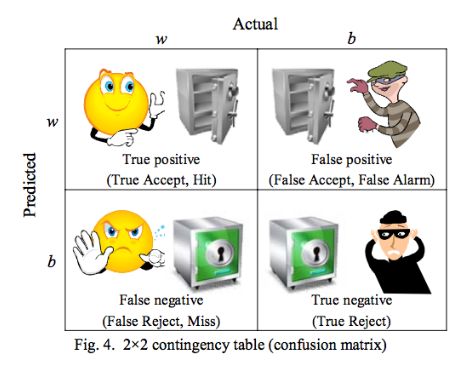
\includegraphics[width=0.75\textwidth]{ChaTappertFig.png}
\caption{\label{contingency_table}Contingency Table (Cha \& Tappert)}
\end{figure}

\begin{figure}
\centering
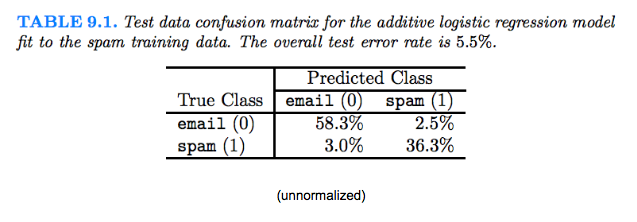
\includegraphics[width=1.0\textwidth]{HTFtable9_1.png}
\label{spam}
\end{figure}

\subsection{Rates}
The ROC curve plots the \textbf{True Positive Rate} (TPR), or sensitivity, against the \textbf{True Negative Rate} (TNR), or specificity.
$$TPR = \frac{TP}{TP + FN}$$
$$TNR = \frac{TN}{FP + TN}$$

Some version of ROC curves use the \textbf{False Positive Rate} (FPR) instead of TNR. When reading an ROC curve remember to always check which convention is used.
$$FPR = \frac{FP}{FP + TN}$$

\textit{Note: $TNR = 1-FPR$}\vspace{2mm}
\newline


\subsection{Accuracy}
\textbf{Accuracy} (ACC) is the number of entities classified correctly over the total number of entities tested. If we denote the total number of positive entities by $P$ and the total number of false entities by $N$ we would get:
$$ACC = \frac{TP+TN}{P+N}$$


\subsection{Precision and Recall}
For datasets that are very skewed (not balanced) TP, FP, TN and FN are not good representations of the performance of the algorithms. In such cases we use:
$$Precision = \frac{TP}{TP+FP}$$
$$Recall = \frac{TP}{TP+FN}$$
$$F-Score = \frac{2}{\frac{1}{Precision}+\frac{1}{Recall}}$$
\textit{Note: F-Score is the harmonic mean of Precision and Recall.}\vspace{2mm}

Document retrieval is an example of a problem with a skewed dataset. Imagine you type in a search query and some algorithm computes a similarity score over a set of stored documents. The threshold you sweep here are the number of results presented to the user. In this scenario:
$$Precision = \frac{|\{\text{Relevant Documents}\}\cap\{\text{Retrieved Documents}\}|}{|\{\text{Retrieved Documents}\}|}$$
$$Recall = \frac{|\{\text{Relevant Documents}\}\cap\{\text{Retrieved Documents}\}|}{|\{\text{Relevant Documents}\}|}$$



\subsection{Receiver Operating Characteristic (ROC) Curve}

The ROC curve is the plot of FPR vs TPR as we vary the classification threshold, and is a graphical means of representing a binary confusion matrix as a function of classifier threshold. The ROC curve is useful because it tells us how good a probabilistic classifier is regardless of specific threshold. Precision and Recall can be plotted together too, similar to the ROC curve.

\begin{figure}
\centering
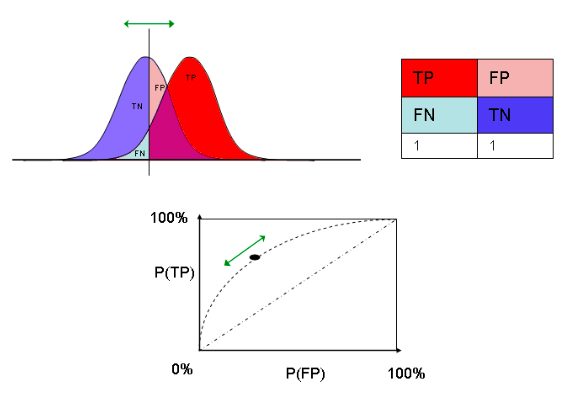
\includegraphics[width=0.75\textwidth]{WikipediaROC.png}
\caption{\label{wikipedia_roc}ROC curve. Top Left: The $x$ axis represents distance or score.  The vertical line represents the classifier threshold setting: scores above the threshold are declared positives. Top Right: 2-class (binary) confusion matrix corresponding to the indicated choice of threshold. Bottom: ROC Curve, with dot representing choice of threshold. Diagonal line represents the ROC curve for random chance.  (Wikipedia)}
\end{figure}

\begin{figure}
\centering
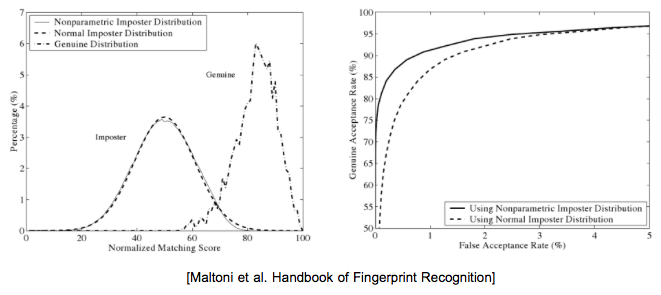
\includegraphics[width=1.0\textwidth]{MaltoniROC.png}
\caption{\label{maltoni_roc}Integrating scores of genuine and impostor pair matches to produce the ROC curve.  As an example, a genuine score would be the similarity between two voiceprints from Alice, while an impostor scores would capture the similarity between a voiceprint form Alice and a voiceprint from Bob.  In general, we expect the distribution of impostor scores to be largely to the left of the genuines, but some overlap is inevitable. (Maltoni et al.)}
\end{figure}

\subsubsection{Area Under the Curve}
A generic metric for comparing the performance of one algorithm to another across all possible thresholds is to compute the Area Under the [ROC] Curve (AUC or AUROC).  This is generic because it summarizes the overall performance, but individual algorithms with lower AUCs could still be more appropriate in certain application contexts. When looking at the value of the AUC, a value of 1/2 corresponds to random guessing, while an AUC = 1 corresponds to perfect prediction. 
\textit{Fun Fact: The AUC is exactly equal to the probability that given two random examples, one positive and one negative, that we give the positive example a higher score.}


\section{Linear Regression}
Last lecture we learned about kNN, which is a \emph{lazy learning} or memory-based method, not dependent on a model fit. In lazy learning algorithms, one defers prediction until query time.  In contrast to this, \emph{eager learning} algorithms, work by summarizing the data using a model or function at training time, and then only rely on the summary model at query time.  To illustrate this, we'll look at a method that is somewhat less lazy than kNN, a method that uses a model, albeit a simple one: linear model fit by least squares.

\subsection{The Linear Model}

The model looks like this:
$${\hat Y} = {\hat \beta}_0+\sum_{j=1}^p X_j{\hat \beta}_j$$
with input vector $X=(X_1,X_2,\ldots,X_p)^\top$ and ${\hat \beta}_0$ the intercept or bias.  The hat on symbols indicates a prediction. \\

To simplify, we can absorb the bias ${\hat \beta}_0$ into the vector of coefficients $X$. $\hat{\beta}$ by adding a constant 1 to the front of $X$.  Then we can write the model very compactly as an inner product:
$$\hat{Y}=X^\top\hat{\beta}$$

Here we have a single outcome variable, so $\hat Y$ is a scalar, but this can be generalized to multiple outputs $Y_1,\ldots,Y_K$ \\

Let $f(X)=X^\top\hat{\beta}$ represent some linear function over the $(p+1)$-dim.\ space. We're going to use this function for classification by applying a threshold to $f(X)$.

\subsection{Fitting with Least Squares}

How do we fit this model?  In this context, \emph{fit} means ``estimate $\beta$.'' The most popular method for doing this is \emph{least squares}.  In this method, we pick $\beta$ to minimize the \emph{residual sum of squares (RSS)}:\footnote{Also referred to as the \emph{sum of squared residuals (SSR)}.}
$$RSS(\beta)=\sum_{i=1}^N(y_i-X_i^\top\beta)^2$$
In other words, we are looking for the best compromise in $\beta$ over all the data points.

We can write this sum in matrix-vector form as:
$$RSS(\beta) = (y-X\beta)^\top(y-X\beta) = \|y-X\beta\|^2$$
where $X\in\mathbb{R}^{N\times (p+1)}$, a matrix where each row is an input vector, and $y\in\mathbb{R}^N$ is a vector of outputs:
$$X=\left[\begin{array}{ccccc}1&X_1^1&X_2^1&\cdots&X_p^1\\1&X_1^2&X_2^2&\cdots&X_p^2\\\vdots& &\vdots& & \vdots\\1&X_1^N&X_2^N&\cdots&X_p^N\end{array}\right] \qquad y=\left[\begin{array}{c}y^1\\y^2\\\vdots\\y^N\end{array}\right]$$
Here we have $N$ data points and $(p+1)$ dimensions. The matrix $X$ is known as the \emph{design matrix}.

We want to find a $\beta$ vector that will best return the desired values of $y$.  How do we solve for $\beta$?  Optimizing with respect to $\beta$ we have,
\begin{align*}
\nabla_\beta SSR(\beta) &= \nabla_\beta \|y-X\beta\|^2\\
0 &= X^\top(y-X\beta)
\end{align*}
also known as ``the normal equations.''  Provided $X^\top X$ is non singular, we have:
$$\hat{\beta}=(X^\top X)^{-1}X^\top y = X^+y$$
where $X^+=(X^\top X)^{-1}X^\top$ denotes the \emph{pseudoinverse} of $X$.

The fitted value for the $i$th input $x_i$ is:
$$\hat{y}_i=x_i^\top \hat{\beta}$$
which is simply the dot product of the input vector with the fitted coefficients.  Importantly, this applies not just for the input points, it applies for an arbitrary input $x_0$, too!  Thus, the linear model \emph{generalizes} over the plane (space, etc.).  How \emph{well} it generalizes, however, is a different story -- we've made some huge simplifying assumptions here, but it's still noteworthy that we're seeing some actual generalization.

\subsubsection{Why Least Squares? (Optional)}

It is worth considering why least squares is such a popular way of defining a ``best'' fit, because it may appear somewhat arbitrary.  Why not minimize the $l_1$-norm or the $\infty$-norm?  Although we might rule out the $l_1$-norm because it lacks differentiability at the minimum, that criticism doesn't carry over to most other norms.

One of the key features that least squares has is that the error nicely decomposes into recognizable quantities.  Similar to the analysis of expected prediction error (EPE) from the previous lecture, we can analyze the expected error of a given model $f(x)$ as follows,
\begin{align*}
E[(f(X) - Y)^2] &= E_X[E[(f(X) - Y)^2 | X]]\\
&= E_X[f(X)^2 -2 f(X)E[Y|X] + E[Y^2|X]]\\
&= E_X[(f(X) - E[Y|X])^2 + E[Y^2|X] - E[Y|X]^2]\\
&= E_X[(f(X) - E[Y|X])^2] + E[var[Y|X]]\\
&= E_X[f(X) - E[Y|X]]^2 + (E[f(X)^2] - E[f(X)]^2) + E_X[var[Y|X]]\\
&= E_X[f(X) - E[Y|X]]^2 + var[f(X)] + E_X[var[Y|X]]
\end{align*}
The three final terms correspond to the squared \emph{bias} of the model with respect to the data ($E_X[f(x) - E[Y|X]]^2$), the \emph{variance} of the model itself ($var[f(X)]$), and the inherent noise in the data ($E_X[var[Y|X]]$).  Clearly, the choice of model $f(x)$ cannot have any effect on this last component.  Minimizing least squares, therefore, puts squared bias on equal terms with model variance. We will talk more about the notion of a \emph{bias-variance trade-off} later.

\subsection{The ``Linear Classifier''}
\label{sec:linclass}
Let's now bring this back to the classification problem from last lecture, with the response $Y$ coded as 0 for blue and 1 for orange; see HTF Fig.\ 2.1.  We use the convention
$$\hat{G}=\left\{\begin{array}{c}\text{orange, if}\quad\hat{Y}>0.5\\\text{blue, if}\quad\hat{Y}\le 0.5\end{array}\right.$$
The \emph{linear decision boundary} in $\mathbb{R}^2$ is given by $\{x:x^\top\hat{\beta}=0.5\}$ and data points in $\mathbb{R}^2$ get the orange label for $\{x:x^\top\hat{\beta}>0.5\}$

\begin{figure}
\centering
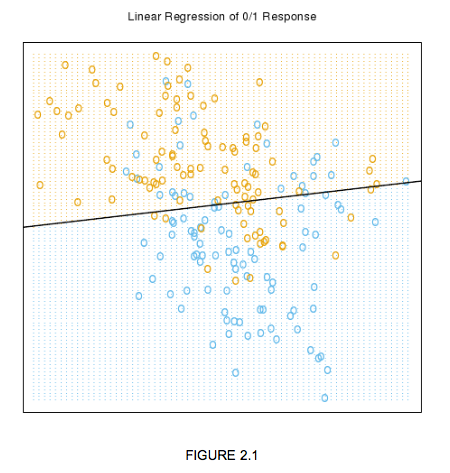
\includegraphics[width=0.75\textwidth]{HTFfig2_1.png}
\end{figure}


How did we do?  We can see the linear model makes a lot of mistakes.  Avoidable?  Yes and no.  One aspect of this approach that should strike us as odd is the binary coding of $Y$ in the face of fitting what amounts to a linear ramp in this case.  Isn't this a strange representation?  We get wildly different contributions to the RSS from pts.\ at varying distance from the decision boundary.

In this sense, linear regression on a $0/1$ response is not very natural.  Soon we'll learn about a more natural way to solve this problem using something called \emph{logistic regression}.

This method is high bias, low variance method. As described by P.~Domingos, ``Bias is a learner’s tendency to consistently learn the same wrong thing. Variance is the tendency to learn random things irrespective of the real signal.'' See Figure \ref{fig:darts} for an illustration of this idea using darts.

\begin{figure}
\centering
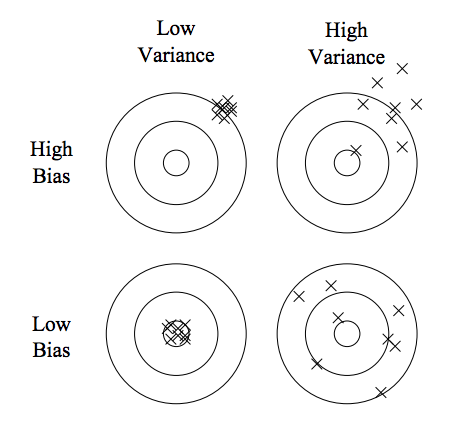
\includegraphics[width=0.5\textwidth]{dartboard.png}
\caption{Bias and Variance in dart throwing. [P.~Domingos 2012]}
\label{fig:darts}
\end{figure}


\end{document}
